\documentclass[10pt,a4paper]{article}
\usepackage[margin=2.2cm]{geometry}
\usepackage{fontspec}
\usepackage{kotex}
\setmainfont{Apple SD Gothic Neo}
\setsansfont{Apple SD Gothic Neo}
\usepackage{amsmath,amssymb}
\usepackage{graphicx}
\usepackage{booktabs}
\usepackage{caption}
\usepackage[dvipsnames]{xcolor}
\usepackage[colorlinks=true,linkcolor=MidnightBlue,citecolor=MidnightBlue,
            urlcolor=MidnightBlue]{hyperref}
\usepackage{titlesec}
\titleformat{\section}{\large\bfseries}{\thesection}{0.6em}{}
\titleformat{\subsection}{\normalsize\bfseries}{\thesubsection}{0.5em}{}
\captionsetup{font=small,labelfont=bf}
\setlength{\parskip}{0.35em}
\setlength{\parindent}{0pt}

\usepackage{mdframed}
\newmdenv[linewidth=0.4pt,linecolor=gray!60,backgroundcolor=gray!5,
          innertopmargin=6pt,innerbottommargin=6pt,skipabove=8pt,skipbelow=8pt]{claimbox}
\newcommand{\claim}[2]{\begin{claimbox}\textbf{주장.} #1\par\smallskip
  \textcolor{gray!70}{\textbf{반증 조건.} #2}\end{claimbox}}

\title{\bfseries 누구의 잘못인가\\[2pt]
\large 아이돌은 부류, 시장팝업은 셋 다 --- 그리고 합동 제거는 어느 쪽에도 답이 아니다}
\author{월드모델 실험실 · 노트 $806$}
\date{2026-08-07}
\begin{document}\maketitle

\section{한 줄}

논문 $168$ 의 선행 시험이다 --- TabPFN 은 \textbf{같은 입력}으로 이겼으므로 결손은
``열이 없어서''가 아니다. 남는 두 가설(합동 적합의 음의 전이 / gbdt 부류의 한계)을
\textbf{단독 F$18$ 팔 하나}로 갈랐다(같은 씨앗 $4{\sim}7$ · A·C 는 노트 $804$ 실측
재사용).

\begin{center}
\begin{tabular}{lrr}
\toprule
& 아이돌 & 시장팝업 \\
\midrule
A 합동 gbdt(챔피언) & $0.4515$ & $0.1545$ \\
\textbf{B 단독 gbdt(새)} & $0.4367$ & $\mathbf{0.0277}$ \\
C 단독 TabPFN & $0.6315$ & $0.2286$ \\
\midrule
$\Delta$전이(A$-$B) & $+0.0148$($2\sigma$ 안) & $\mathbf{+0.1268}$($5.4$배) \\
$\Delta$부류(C$-$B) & $\mathbf{+0.1948}$($5.3$배) & $\mathbf{+0.2009}$($8.6$배) \\
\bottomrule
\end{tabular}
\end{center}

\textbf{아이돌은 (ㄴ) 부류가 답}이고 \textbf{시장팝업은 (ㄹ) 합동이 돕는 곳}이다
--- 둘 다 사전 예측의 주 갈래대로다(이 세션 첫).

\begin{figure}[t]\centering
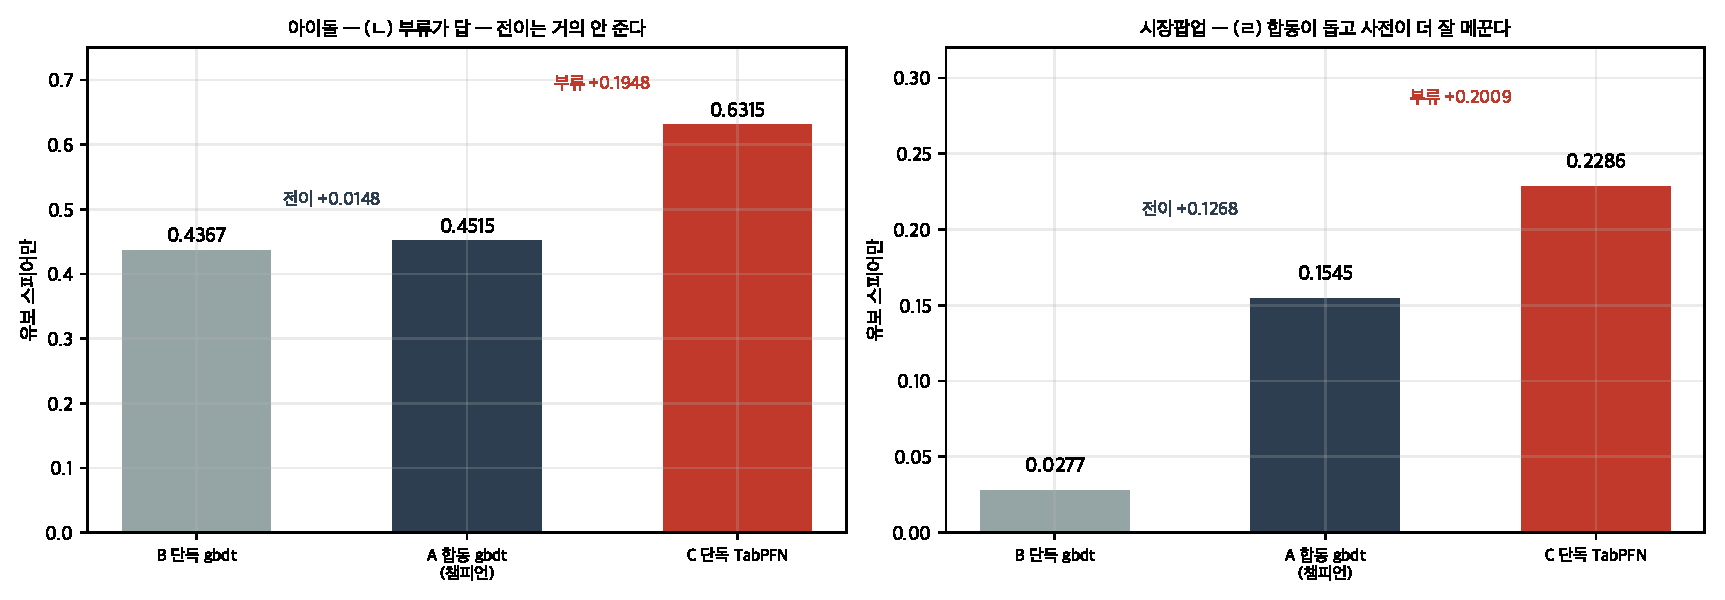
\includegraphics[width=0.92\textwidth]{figs/blame.pdf}
\caption{같은 세 팔, 다른 두 답 --- 전이 화살과 부류 화살의 크기를 보라.}
\end{figure}

\section{두 도메인, 두 기제}

\claim{\textbf{아이돌($122$행 · $15$열): gbdt 는 어떻게 적합해도 $0.44{\sim}0.45$
다.} 합동을 빼도 안 내려간다($-0.0148$ · $2\sigma$ 안) --- 전이는 이 도메인에 거의
아무것도 안 주고 있었고, TabPFN 의 $+0.19$ 는 순수하게 \textbf{모형 부류(SCM
사전·문맥 내 베이즈)의 우위}다.}
{\textbf{시장팝업($123$행 · 살아 있는 열 $3$개)은 정반대다} --- 단독 gbdt 는
\textbf{거의 무신호($0.0277$)}이고 합동이 $+0.127$ 을 끌어올린다. 그런데 같은
$3$열로 사전은 $0.2286$ 을 낸다 --- \textbf{전이도 사전도 각자 방식으로 $3$열의
부족을 메꾸는데 사전이 더 잘 메꾼다.} 이 도메인의 진짜 처방은 헤드도 전이도
아니라 \textbf{열}일 수 있다 --- 살아 있는 열 $3$개는 배선의 문제이고, 그것이
늘면 세 팔이 다 오를 것이다(안 쟀다).}

\section{처방의 확인}

\claim{\textbf{``합동 제거''는 어느 쪽에도 답이 아니다} --- 아이돌에선 무의미하고
($\Delta$전이 $\approx 0$) 시장팝업에선 해롭다($-0.127$). 논문 $168$ 의 처방
(\emph{합동 유지 + 소외 도메인 보조 헤드})이 \textbf{기제 수준에서 확인됐다.}
챌린저 장부(\texttt{lab/challenger.py})에 기제 문단을 갱신했다.}
{남는 승격 문제: 아이돌·시장팝업에는 집 밖 짝이 없어 규약 $12$ 를 그대로 적용할
수 없다. \textbf{서빙에 물리려면 대체 검증(전향 봉인 채점 등)의 절차 설계}가
필요하고 그것이 T$1$ 의 남은 갈래다.}

\end{document}
